
\chapter{Data analytics}

In this chapter I propose three hypotheses. They are:

\begin{enumerate}
  \item Skedge's differences from and additions to CDCS are \textbf{usable and have real need}.

  \item Skedge’s \emph{navigations-per-add} demonstrate the \textbf{effectiveness of its search features} for each of the following three user search paradigms:

  \begin{enumerate}
    \item direct search,
    \item exploratory search, and
    \item peer-guided search
  \end{enumerate}

  \item Skedge’s \textbf{DSQL is user-friendly}; users learn more advanced search types over time \textbf{simply by using it}.
\end{enumerate}

\noindent In the following sections I will present my analysis on collected usage data since November 3rd 2015, which will serve to validate each hypothesis.

\section{Usage}

\subsection{General}

From November 3, 2015 to April 11, 2016 (a period of 159 days), Skedge has seen\ldots

\begin{itemize}
  \item 4,713 users that have added or bookmarked at least 1 course
  \item 5,256 schedules
  \item 17,012 sessions\footnote{A session is defined by a period of activity expiring after 30 minutes of inactivity}, 75\% of which are from returning visitors
  \item 107 sessions per day, on average
  \item 5.40 pages viewed per session, on average 
  \item 6 minutes spent per session, on average
\end{itemize}

\begin{figure}
  \centering

  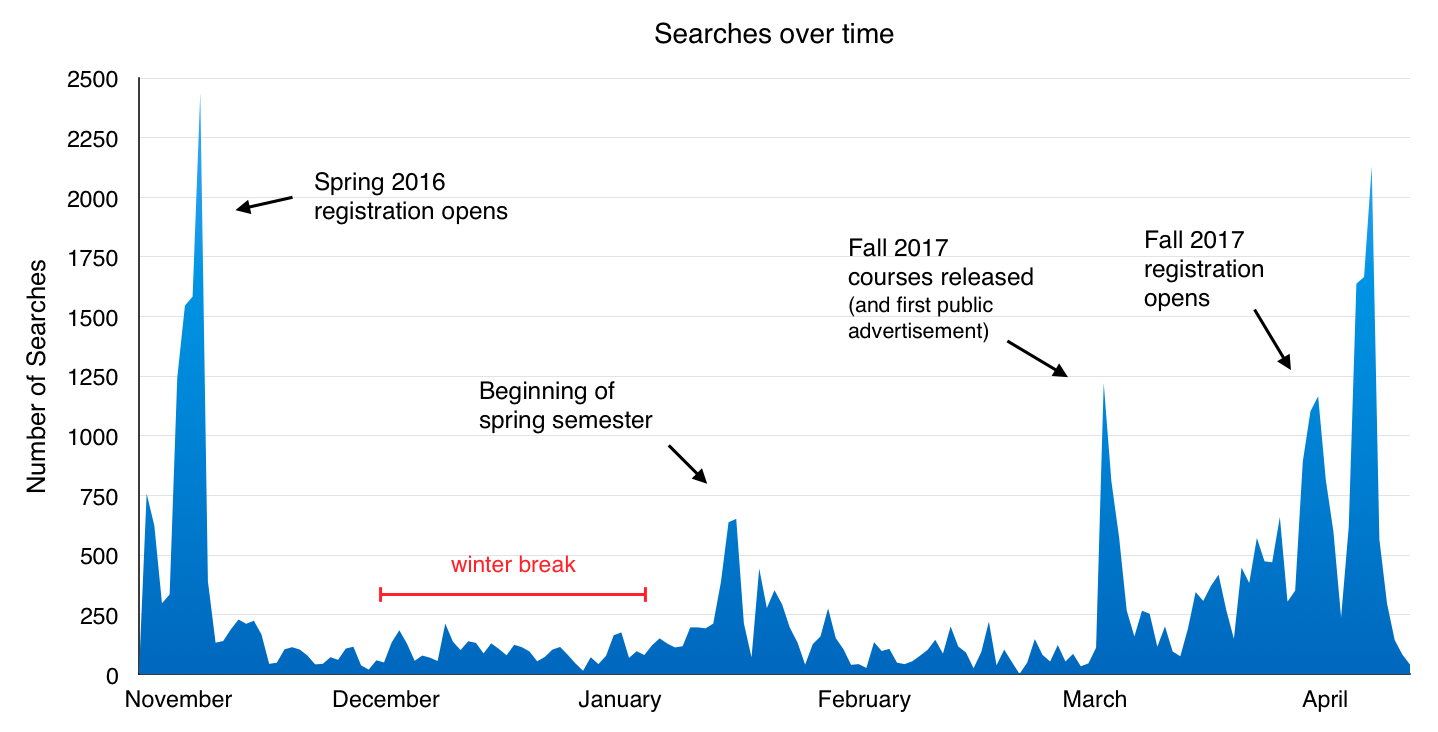
\includegraphics[width=1.0\textwidth]{images/graph/searches}

  \caption{Etc}
  \label{fig:searches}

\end{figure}

periodic visit cycle graph means people are actually using it and decided to stay with it, not declining, can be seen w exports & link-searches.

also should be noted that NO seniors participated in the last, the majority of the userbase!

success Considering skedge is OPTIONAL.

\subsection{Exports}

\begin{figure}
  \centering
  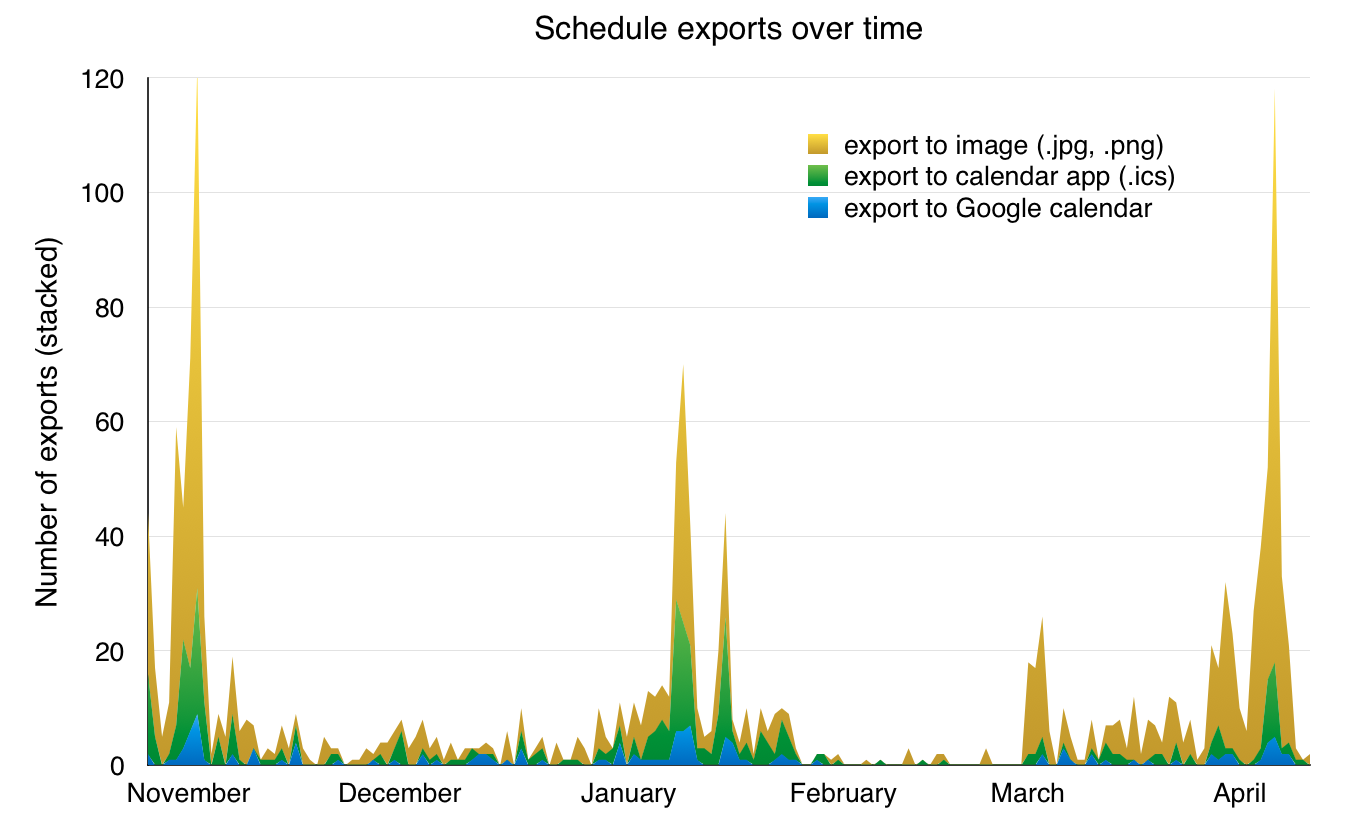
\includegraphics[width=1.0\textwidth]{images/graph/exports}

  \caption{Etc}
  \label{fig:searchtypes}
\end{figure}

Success! (broken on cdcs)

\subsection{``Link-searches''}

\begin{figure}
  \centering
  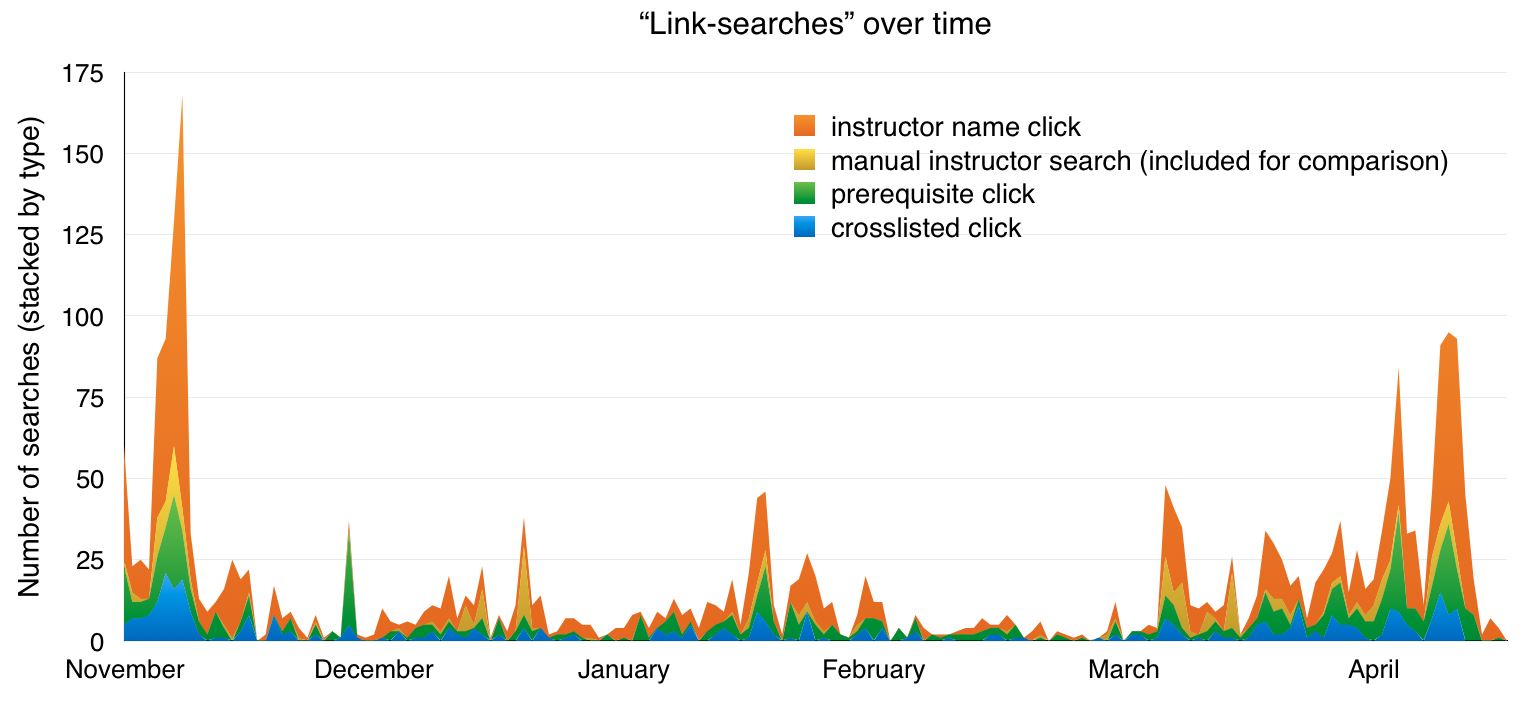
\includegraphics[width=1.0\textwidth]{images/graph/linksearches}

  \caption{Etc}
  \label{fig:searchtypes}
\end{figure}

Success, used!

\subsection{Mobile}

\begin{itemize}
  \item 11.54\% of sessions
  \item 2.74 page viewed per session, on average
  \item 2 minutes spent per session, on average
\end{itemize}

success bc mobile doesn't exist on cdcs

\subsection{Course Blocks}

\begin{figure}
  \centering

  \fbox {
    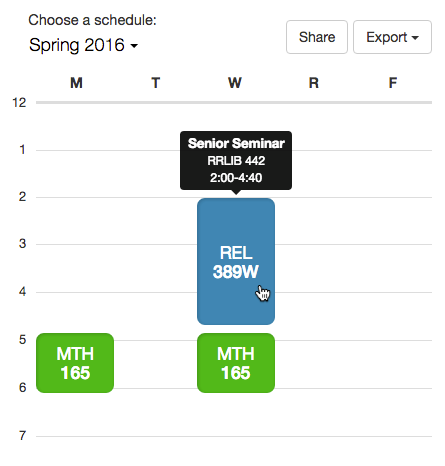
\includegraphics[width=8cm]{images/skedge/blocks}
  }

  \caption{Etc}
  \label{fig:searchtypes}

\end{figure}

40\% of sessions have at least one block-click
Average of 5.12 block-clicks per session

success because you can't click schedule blocks in better cdcs!!

\subsection{Search}

  \subsubsection{Search types}

  \begin{figure}
    \centering
    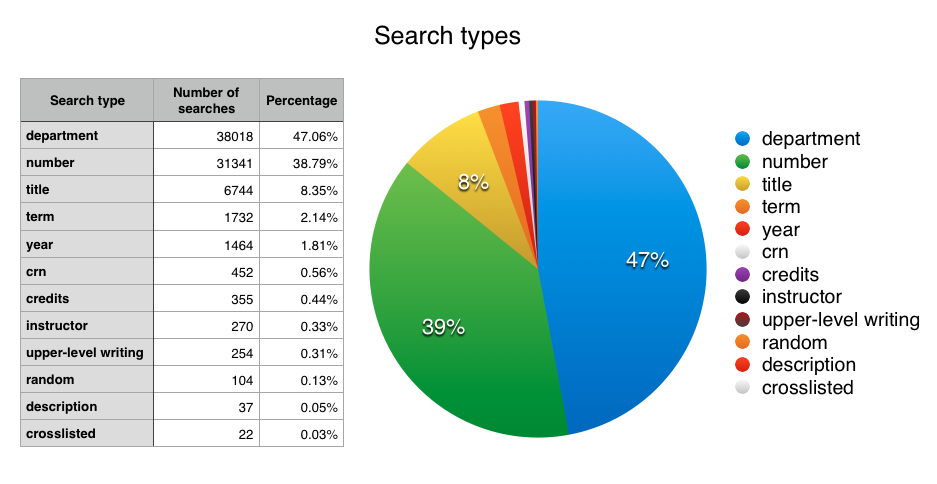
\includegraphics[width=1.0\textwidth]{images/graph/searchtypes}

    \caption{Etc}
    \label{fig:searchtypes}

  \end{figure}

  \subsubsection{Empty searches}

  Can learn from these
  Some funny ones


\section{Effectiveness of search}

\subsection{Definitions}

A navigation is defined as
a search, or
a click on an instructor’s name, or
a click on a crosslisted or prerequisite course link

The navigations-per-add measure is
the number of navigations a user took (within one session) until a course was added, bookmarked

\subsection{Trends}

\begin{figure}
  \centering
  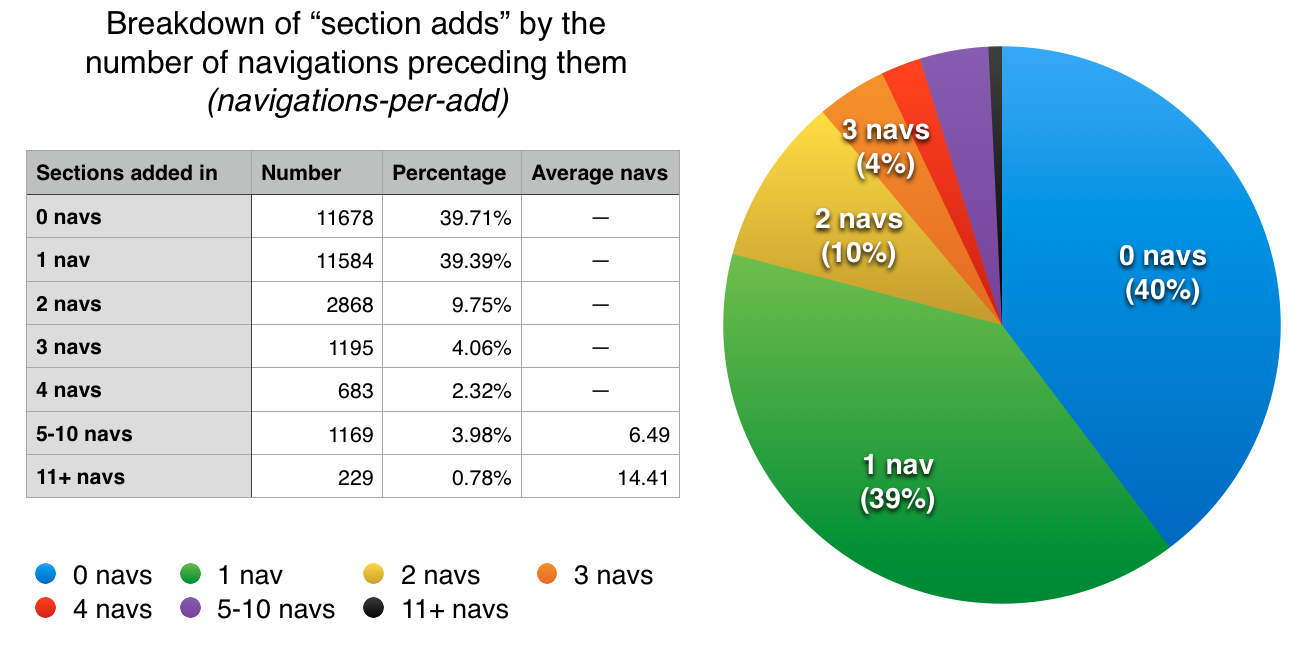
\includegraphics[width=1.0\textwidth]{images/graph/combined_navs}

  \caption{Etc}
  \label{fig:searchtypes}
\end{figure}

\subsection{Breaking them apart}

  behavioral patterns
  Direct search for specific course
  Discovery, browsing, exploring

  \subsubsection{Direct searches}

  \begin{figure}
    \centering
    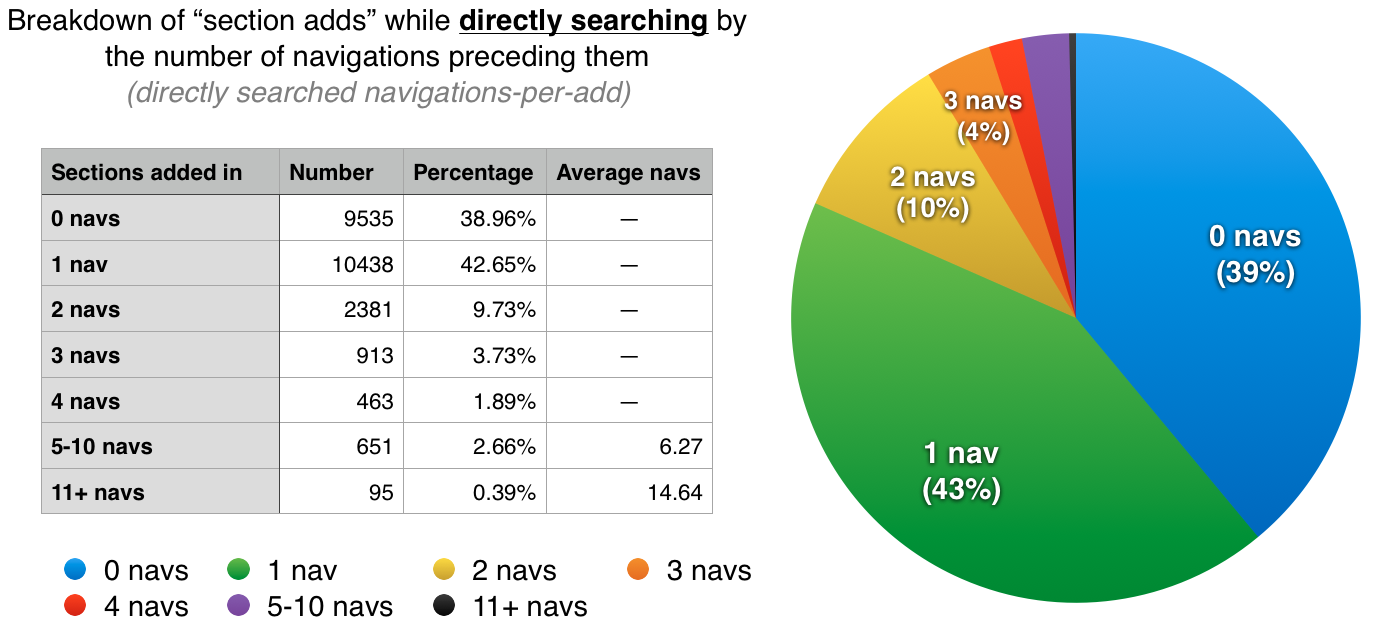
\includegraphics[width=1.0\textwidth]{images/graph/direct_navs}

    \caption{Etc}
    \label{fig:searchtypes}
  \end{figure}

  Why would 0-navs be so common with direct searches? 65\% subsections!

  \subsubsection{Browse}

  % STAT: Find major of users, find how many non-major courses they found

  \begin{figure}
    \centering
    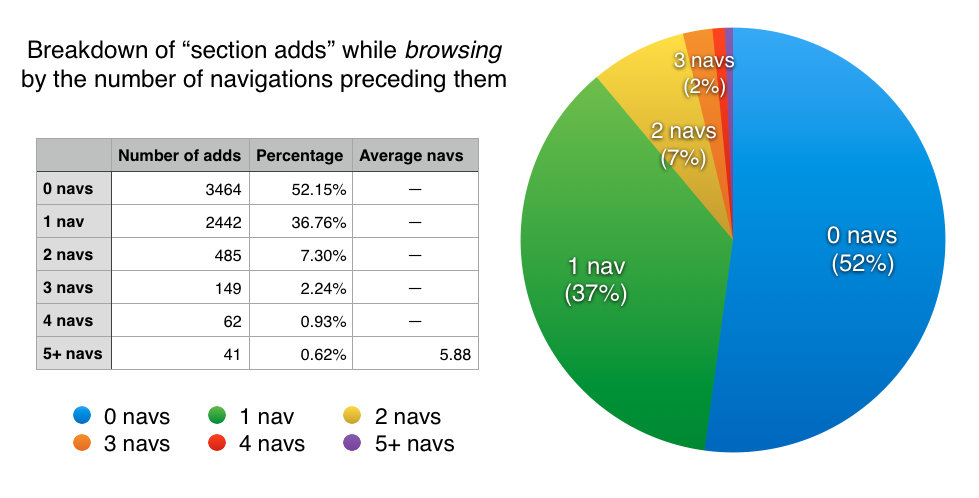
\includegraphics[width=1.0\textwidth]{images/graph/browse_navs}

    \caption{Etc}
    \label{fig:searchtypes}
  \end{figure}

  As expected, the 0-navs were mostly maincourses

  Effective++

  \subsubsection{Social}

  90 users have linked Skedge to Facebook
  Since March 1st,
  4,000+ visits (200 visits/day)
  ~60\% of visits to /social were returning visitors
  90 overlays onto friends’ schedules
  10 clicks to Facebook profiles :(
  - get stats from the fb dashboard

  success?????


\section{Complexity of users' searches over time}

\subsection{Definitions}

Points for search by (omits number and dept.):

description
credits
crosslisted
CRN
instructor
title
year
term
‘random’
upper-level writing

“CSC” → 0
“MTH 165” → 0
“taught by hema” → 1   ✓    (2 searches) 
“random mur 1-2 credits” → 2   ✓    (1 search) 


\subsection{Trends}

\begin{figure}
  \centering

  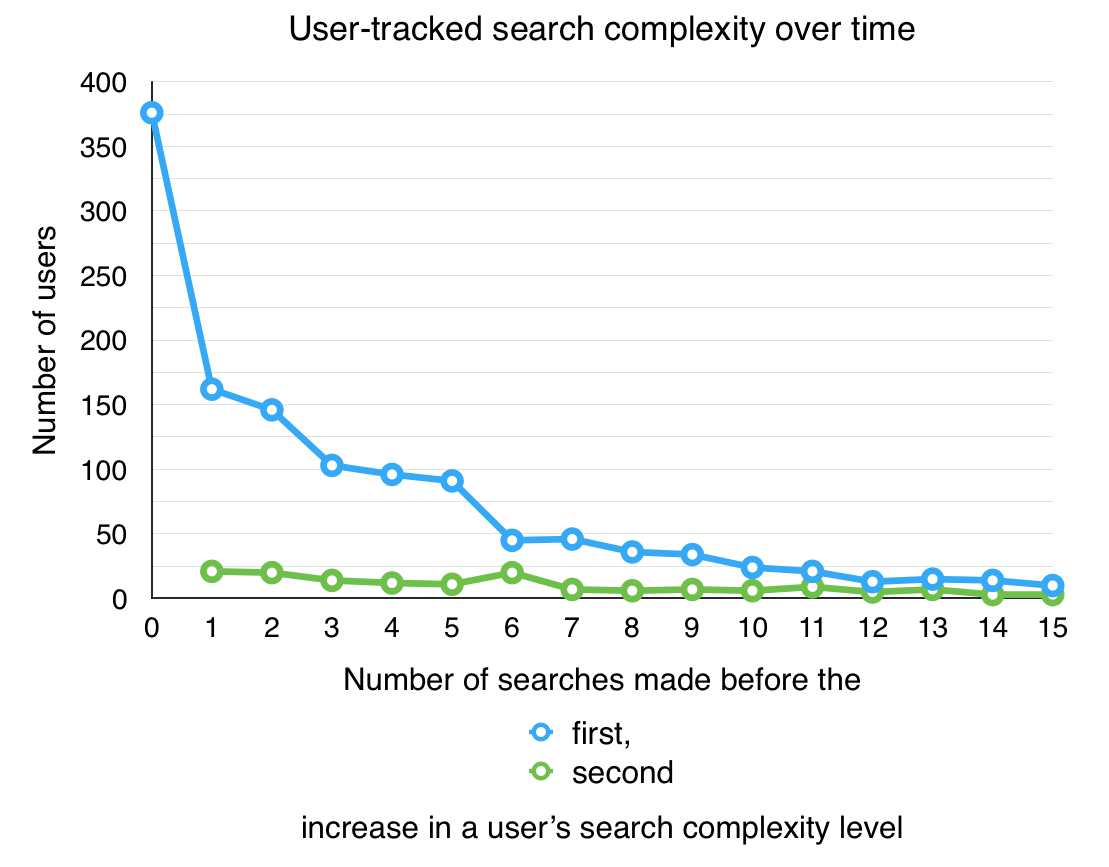
\includegraphics[width=1.00\textwidth]{images/graph/search_dt}

  \\
  \vspace{5pt}

  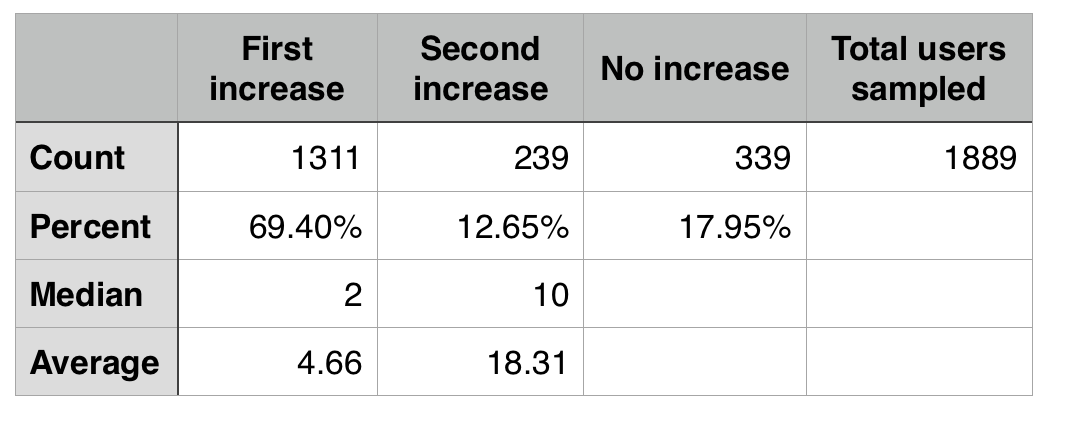
\includegraphics[width=0.65\textwidth]{images/table/search_dt}

  \caption{Etc}
  \label{fig:searchtypes}
\end{figure}

First increase (60.5\% of users)
Median: 2 searches
Average: 4.23 searches
(Starting at 1 counts as an increase value of 0)

Second increase (7.9\% of users)
Median: 8 searches
Average: 17.52 searches

DSQL++